\section{Dark bubbles from string theory: An explicit construction}\label{sec: db_from_st}
\textcolor{red}{I GUESS THAT HERE I NEED TO WRITE A GOOD SUMMARY OF THE MODEL I WILL USE (OSCAR'S). SPECIALLY WHAT IT WAS USED FOR IN THE PAST AND HOW GOOD IT MAY CONNECT TO THE KIND OF SCENARIO WE HAD IN MIND FOR BUBBLES.}

\textcolor{red}{EMPHASISE THAT THE STACK OF BLACK BRANES IS A BLACK HOLE IN HIGHER DIM.}
\subsection{A black hole in the bulk: Ten-dimensional Kerr or five-dimensional Reissner-Nordström one?}
Let us start by defining the parametric coordinates that will be used to describe the 10 dimensional rotating background\footnote{It is important to notice the choice of $z$ to describe the $\text{AdS}_{5}$ throat direction. Spoiler alert: There will be a convenient change of coordinates soon to adequate $r$-direction. Stay alert.}:
\textcolor{red}{OBSERVE THE CHANGE OF COORDINATE DEFINITION WRT THE PAPER. SO THE RESULTING EQUATIONS ARE MORE FAMILIAR WITH THE USUAL THROAT.}
\begin{equation}\label{eq: 10D_coordinates}
	x^{\mu} = \{t, \alpha, \beta, \gamma, z, \theta, \psi, \phi_{1},\phi_{2},\phi_{3}\},
\end{equation}
and its line invariant
\begin{equation}\label{eq: 10Dmetric}
  \text{ds}_{10}^2= \text{ds}_5^2 + L^2 \sum_{i=1}^3 \left\{ \dpar\sigma_i^2 + \sigma_i^2 \left( \dpar\phi_i + \tfrac{1}{L} A(z) \right)^2 \right\},
\end{equation}
where $A(z)$ is a 10 dimensional one-form that will be later discussed and the $\sigma_i$-functions are combinations of trigonometric functions of two angles\footnote{\textcolor{red}{ADD REF AND COMMENTS ABOUT THE PROCEDENCE OF THIS ANGLES (from where to where do they run) AND PROBABLY, COMMENTS ABOUT THE SPHERE?}} $\{\theta, \psi$\} of the $S^{5}$ as:
\begin{equation}
 \sigma_1 = \sin\theta \ , \qquad \sigma_2 = \cos\theta \sin\psi \ , \qquad \sigma_3 = \cos\theta \cos\psi \ .
\end{equation}
As introduced in section \ref{sec: simple_example}, $L$ is the $\text{AdS}_{5}$ radius in Eq. (\ref{eq: 10Dmetric}). It is important to notice that this radius also sets the scale of the extra compact dimensions of $S^{5}$. This can already raise some eyebrows, as it points to lack of scale separation, as discussed in [SEC Landscape]. However, this will be a key signature of the dark bubble embedding into supegravity, as this model acquires the aforementioned scale separation via tension-to-charge ratio instead. We will later explore this method in section \ref{subsec: energy_scale}. 

Conducting our attention back to the line invariant (\ref{eq: 10Dmetric}), we can define the five dimensional asymptotically-AdS metric $\text{ds}_{5}$ as:
\begin{equation}\label{eq: 5DmetricQ}
  \text{ds}_{5}^{2} = - h(z)^{-2} f(z) \dpar t^{2}
        + h(z) \big[ f(z)^{-1} \dpar z^{2} + z^{2} \dpar \Omega_{3}^{2} \big] \ ,
\end{equation}
where $d\Omega_{3}^2$ is the usual unit metric of the 3-sphere [ref to COSMO SECTION]. The radial functions $h(z)$ and $f(z)$ are expressed as
\begin{equation}\label{eq: h_and_f_bh}
    \begin{split}
        h(z)&=1+\frac{q^{2}}{z^{2}} \ , \\
 f(r) &= 1 - \frac{m}{z^{2}} + \frac{z^{2}}{L^{2}} h(z)^{3},
    \end{split}
\end{equation}
where $m$ and $q$ are respectively the mass and charge of the five dimensional black. Wait? What five-dimensional black hole? Let us then perform a "massage" to Eqs. (\ref{eq: 5DmetricQ}, \ref{eq: h_and_f_bh}) to provide a more familiar black hole-ish line invariant. One can start this task by performing a simple change of coordinates, defining a new radial coordinate $r$ as:
\begin{equation}\label{eq: change_coordinates}
    r^{2} = z^{2}h(z) = q^{2} + z^{2} .
\end{equation}
This change of coordinates will substantialy transform Eq. (\ref{eq: 5DmetricQ}), yielding:
\begin{equation}\label{eq: metricargument}
    \text{ds}_{5}^{2} = -g(r) \dpar t^{2} + g(r)^{-1} \dpar r^{2}+r^{2} \dpar \Omega_{3}^{2}, \qquad \quad g(r) = 1 + k^{2}r^{2}- \frac{2\kappa_{5} M}{r^{2}} + \frac{\kappa_{5}^{2} Q^{2}}{r^{4}}, 
\end{equation}
with 
\begin{align}\label{eq: identifications_MQ}
    M = \frac{1}{2\kappa_5}\left(m + 2q^2\right), &&  Q^2 = \frac{1}{\kappa_5^2}q^2(m+q^2),
\end{align}
with $\kappa_5 = 8\pi G_5$. It is now easy to see that the change of variables described in Eq. (\ref{eq: change_coordinates}) casts the line invariant (\ref{eq: 5DmetricQ}) in the familiar form\footnote{The patch we are describing with the metric (\ref{eq: 5DmetricQ}) corresponds to the requirement $r\geqslant q$. This is actually not an issue since the  horizon $r_{H}$ will be covered by the patch.} of a five dimensional Reissner-Nordström black hole living in an $\text{AdS}$ vacuum [REF]. Observe that, for a small black hole, with $r_{H} \ll L$, we recover a flat space description and it is required $Q<M$ to get a horizon and no naked singularity. On the other hand, if we want to study a horizon larger that the $\text{AdS}_{5}$ radius, this immediately implies $Q\ll M$.

Let us recap now the interpretation of both ten and five dimensional geometries. In the ten dimensional approach, we will observe a Kerr black hole which rotates in three of the compact directions of $S^{5}$ (i.e. $\{\phi_{i}\}$). When we zoom out and not have resolution of the five dimensional sphere, the black hole no longer rotates. It becames "static" from the point of view of a five dimensional observer, but it acquires a charge $q$ due to its motion in the compact directions (This will be further explained later). This charge becomes effective (i.e. charge $Q$) when the change of coordinates (\ref{eq: change_coordinates}) is performed to recover the more familiar description of a Reissner-Nordström black hole living in $\text{AdS}$.

As it is well known, this type of black holes enjoy two different horizons [REFS to book]: The \textit{outer} horizon (i.e. event horizon) and the \textit{inner} one (i.e. the Cauchy horizon). When these two horizon become degenerate (i.e. $r_{H} = r_{h}$), this corresponds to an extremal black hole description. We will not further discuss charged black holes and their connection to the weak gravity conjecture here (see [SWAMP] for more details), but, for computational purposes in the incoming sections, we find more convenient to express (\ref{eq: metricargument}) in terms of the two aforementioned horizons: $\left\{r_{h}, r_{H}\right\}$ as the inner and outer horizons. In this way, we can express $g(r)$ in Eq. (\ref{eq: metricargument}) with the following Ansatz:
\begin{equation}\label{eq: horizon_ansatz}
    g(r) = \frac{k^{2}}{r^{4}}\left(r^{2} + c\right)\:\left(r^{2} -r_{h}^{2}\right)\:\left(r^{2} - r_{H}^{2}\right),
\end{equation}
with $c \in \mathbb{R}$. A simple match between Eqs. (\ref{eq: metricargument}, \ref{eq: horizon_ansatz}) shows that:
\begin{equation}\label{eq: MQhorizons}
    \begin{split}
        &M= \frac{1}{2 \kappa_{5}}\left[r_h^{2} + r_H^{2} +k^{2} \left( r_{h}^{4}  + r_h^{2} r_H^{2}  + r_H^4 \right)\right],  \\
    &Q^2 =\frac{r_{h}^{2}\:r_{H}^{2}}{\kappa_5^2} \:\left[1 + k^{2}\left(r^{2}_{h}+ r_{H}^{2}\right)\right],\\
    &c = r_{h}^{2} + r_{H}^{2} + \tfrac{1}{k^{2}}.
    \end{split}
\end{equation}
which simplifies when the black hole is extremal. Let us keep in mind these identifications for future section and conduct our attention back to the one-form potential $A(z)$ in Eq. (\ref{eq: 10Dmetric}). This form acts as a gauge field from the 5D point of view \textcolor{red}{WHY?}. In term of the old coordinates (i.e. $\{t, \alpha, \beta, \gamma, z\}$) it can be written as:
\begin{equation}\label{eq: gaugepot_A}
 A(z) = \frac{q}{z_H^2+q^2}\sqrt{ \left(q^2+z_H^2 \right) + \frac{z_H^4}{L^2} h(z_H)^3} \left(1-\frac{z_H^2+q^2}{z^2+q^2}\right) \dpar t.
\end{equation}
Observe that gauge freedom has been summoned to add a constant that sets $A(z_H) = 0$. This is required as a $A(z)$ is temporal gauge potential, and must vanish at the horizon. This potential can be expressed in a more handable way in two steps:
\begin{enumerate}
    \item Part of the argument of the root in Eq. (\ref{eq: gaugepot_A}) is the mass $m$ of the black hole\footnote{This can be easily obtained by computing the outer horizon in Eq. (\ref{eq: 5DmetricQ})}. This is:
    \begin{equation}
        m = z_{H}^{2}\left(1 + \frac{z_{H}^{2}}{L^{2}}h(z_{H})^{3}\right).
    \end{equation}
    \item Furthermore, performing the change of variables (\ref{eq: change_coordinates}) and making use of the identifications (\ref{eq: identifications_MQ}) to further simplify in the new coodinate system, one obtains:
    \begin{equation}\label{eq: gaugepot_A_new_coordinates}
        A(r) = \kappa_{5} Q \left(\frac{1}{r_{H}^{2}} - \frac{1}{r^{2}}\right).
    \end{equation}
\end{enumerate}
The stack of rotating $D_{3}$-branes in the ten dimensional background will source the self dual $F_{5}$ Ramond-Ramond (RR) field strength, which can be written in terms of the radial function $h(z)$ and the one-form $A(z)$. However, what we will need for future computations is the corresponding four-form potential $C_{4}$, with $\dpar C_{4}=F_{5}$. This is:
\begin{equation}\label{eq: C4_pot_old}
C_4 (z, z_{H}, q) = \frac{1}{L}\left[(z^2+q^2)^2 - (z_H^2+q^2)^2\right] \dpar t \wedge \epsilon_3 + L^2 q \: \sqrt{ z_H^2 + q^2 + \frac{z_H^4}{L^2} h(z_H)^3}\ \sum_i \sigma_i^2\, \dpar \phi_i \wedge \epsilon_3 \ ,
\end{equation}
where $\epsilon_{3}$ corresponds to the volume-form associated with $\dpar \Omega_{3}$ in Eq. (\ref{eq: 5DmetricQ}). Following the same recipe describe above, one cast the four-form $C_{4}$ in terms of the new variables as:
\begin{equation}\label{eq: C4_pot_new}
    C_4 (r, r_{H}, Q) = \underbrace{\frac{1}{L}\left[r^4 - r_{H}^{4}\right]}_{(C_{4})_{t}} \dpar t \wedge \epsilon_3 + \underbrace{L^2 \: \frac{Q}{\kappa_{5}} \sum_i \sigma_i^2\, \dpar \phi_i}_{(C_4)_{\phi}=\sum_i(C_4)_{\phi_i}} \wedge \epsilon_3.
\end{equation}
Observe that we have split the four-form $C_{4}$ into its time-dependent and $\phi_{i}$-dependent pieces. This notation will further simplify computations to come. 

With this we finish the black hole description, both from ten and five dimensional perspectives. Let us now explore the explicit embedding of the $D_{3}$-brane in the ten dimensional ambient space.

\subsection{The $D_{3}$-brane dynamics}
Let us now move on and study the motion of a nucleated $D_{3}$-brane. The starting point of such enterprise is the action governing its dynamics:
\begin{equation}\label{eq: D3_action}
  S_{D_{3}} = S_{\text{DBI}} +S_{\text{WZ}} =  -T_3\int \dpar^4\xi \sqrt{-\det P[G]}+T_3\int P[C_4].
\end{equation}
The Dirac-Born-Infeld (DBI) term will be in charge of describing the geometrical features of the embedding, while the Wess-Zumino (WZ) term with $C_4$ captures the non-gravitational forces on the brane due to fields external to it. $P[\dots]$ denotes the pullback of spacetime fields to the world volume of the brane. This is no more than the projection of ten-dimensional coordinates onto the three-dimensional geometry of the $D_{3}$-brane, with tension $T_{3}$. These, the brane's embedding functions will be denoted by capital versions of the spacetime coordinates: $\mathcal{X}^\mu(\xi)$. In this set up, we will set the dilaton $\phi$ constant \textcolor{red}{WHY?}.

The dynamical description of the branes is as follows: The stack of $D_{3}$-branes, and hence the nucleated one, wrap the three-sphere $\dpar {\Omega_{3}}$ inside the $\text{AdS}_5$ piece of the metric, with the radial $r$-coordinate (hence $\mathcal{R}$) depending only on the time component. The ten dimensional black hole in the background rotates in the azimuthal $\phi_i$-directions on $S_{5}$. This implies that a $D_{3}$-brane escaping from the stack will preserve a portion of the angular momentum of this. Therefore, it will also move in those directions. Let us, for the sake of simplicity in the construction of this model, set the three angular momenta associated to each $\phi_i$-directions equal in the background. This implies that the brane will rotate with the same angular velocity in all $\phi_i$ directions. Finally, we will assume a constant position in the remaining coordinates of the compact $S_{5}$, i.e. $\{\Psi = \psi_{0}, \, \Theta = \theta_{0}\}$. The brane's embedding functions are then given by:
\begin{equation}
  \mathcal{T}=\mathcal{T}(\tau) \, , \qquad \mathcal{R}=\mathcal{R}(\tau) \, , \qquad \Theta = \theta_0 \, , \qquad \Psi = \psi_0 \, , \qquad \Phi_1 = \Phi_2 = \Phi_3 = \Phi(\tau) \ .
\end{equation}
Here, although we write $\tau$ as a time parameter on the induced geometry, we do not yet specify if it denotes its proper time. We will later see that this is case. From the point of view of an observer living in $\text{AdS}_5$, the rotation translates into an effective charge $Q$ under the gauge field $A$. When a brane nucleates, carrying a portion of the charge, it will also effectively lower the charge of the remaining black hole.

Before we start to analyse the action (\ref{eq: D3_action}), we need some more practical notation. Derivatives with respect to $\tau$ will be denoted by a dot. The components of the ten dimensional metric (\ref{eq: 10D_coordinates}) will be denoted by $G_{\mu\nu}$. It will also be useful to define the mixing of the azimuthal-time and azimuthal-azimuthal components in the compact piece of Eq. (\ref{eq: 10D_coordinates}) as $G_{t\phi}=\sum_i G_{t\phi_i}$ and $G_{\phi\phi}=\sum_i G_{\phi_i\phi_i}$ respectively.

Let us start the analysis of Eq. (\ref{eq: D3_action}). The pullback $P[G]$ is no more than the induced $g_{\tau\tau}$-metric entry of the expanding $D_{3}$-brane. This is:
\begin{equation}\label{eq: pullback_G}
    P[G] = g_{\tau\tau} = G_{tt} \dot \T^2 + G_{rr} \dot \R^2 + 2G_{t\phi} \dot \Phi \dot \T + G_{\phi\phi} \dot\Phi^2.
\end{equation}
This is also the square of the velocity that a comoving observer living on the brane will experiment,
\begin{equation}\label{eq: 10velocity}
 \dot X^2 = \dot X_\mu \dot X^\mu = G_{tt} \dot \T^2 + G_{rr} \dot \R^2 + 2G_{t\phi} \dot \Phi \dot \T + G_{\phi\phi} \dot\Phi^2 \ ,
\end{equation}
with
\begin{equation}
    \dot X \equiv \frac{\partial X^\mu}{\partial\tau}\partial_\mu = \dot \T \partial_t + \dot \R\, \partial_r + \dot \Phi\sum_{i=1}^{3} \,\partial_{\phi_i} \ .
    \end{equation}
The induced line element on the brane worldvolume is:
\begin{equation}
 \dpar s^2_4 = \dot X^2 \dpar \tau^2 + \R(\tau)^2 \dpar \Omega_{3}^2 \ .
\end{equation}
Now one can see that picking $\tau$ to be the proper time of an observer living on the brane would set $\dot{X}^2=-1$, and the induced metric takes the usual FLRW-form, with $\R(\tau)$ acting as the scale factor.

Similarly, the pullback of the four-form $C_{4}$ is:
\begin{equation}\label{eq: pullback_C4}
    P[C_{4}] = \left((C_{4})_{t} \frac{\partial \T}{\partial\tau} + \sum_{i} (C_{4})_{\phi} \frac{\partial \Phi_{i}}{\partial\tau}\right)\dpar \tau \wedge \epsilon_{3}.
\end{equation}

Finally, the action (\ref{eq: D3_action}) can be rewritten as:
\begin{equation}\label{eq: Lag_density_action}
    S_{D_{3}} \equiv \int d\tau \mathcal{L}_{D_{3}}  = -2\pi^2 T_3 \int d\tau \left\{ \R^3 \sqrt{ -\dot X^2 } - (C_4)_t \dot\T - (C_4)_{\phi} \dot\Phi \right\},
\end{equation}
where $\mathcal{L}_{D_{3}}$ represents the Lagrangian density of the $D_{3}$-brane. Observe that integration over the $S^3$ has been already taken into account. As one can notice, the Lagrangian density does not depend on the time component $\T$ or the angular coordinates $\Phi_{i}$, just their derivatives. This points to conserved quantities in the system. For our obscure purposes,\footnote{i.e. to make our computations as simple as possible.} let us define the conserved angular momentum
\begin{equation}
 J \equiv \frac{1}{2\pi^2 T_3}\frac{\dpar\mathcal{L}_{D_{3}}}{\dpar \dot\Phi} = \frac{\R^3 }{\sqrt{ -\dot X^2 }} \left(G_{t\phi} \dot\T + G_{\phi\phi} \dot\Phi \right) + (C_4)_\phi.
\end{equation}
With this, let us Legendre transform to substitute $\dot\Phi$ for $J$, automatically satisfying $\Phi$'s EoM. Additionaly, let's define $J_C = J-(C_4)_\phi$, which we will give a physical interpretation later. We then obtain \textcolor{red}{why do we choose positive root?}:
\begin{equation}
 \dot\Phi = -\frac{G_{t\phi}}{G_{\phi\phi}}\dot\T \pm J_C \sqrt{\frac{\left(\frac{G_{t\phi}^2}{G_{\phi\phi}^2}-\frac{G_{tt}}{G_{\phi\phi}} \right) \dot\T^2 - \frac{G_{rr}}{G_{\phi\phi}} \dot\R^2 }{\left(\R^6\, G_{\phi\phi} + J_C^2\right)}}.
\end{equation}
and the Legendre transformation becomes:
\begin{equation}\label{eq: Lag_Legendre}
\begin{split}
 \mathcal{L}_{D_{3}}^J &= \mathcal{L}_{D3} - \dot\Phi J \\
 &= -2\pi^2 T_3 \dot\T \left\{-(C_4)_t  - \frac{G_{t\phi}}{G_{\phi\phi}}J_C  + \sqrt{-\left(\R^6 + \frac{J_C^2}{G_{\phi\phi}}\right) \left( \underbrace{G_{tt}-\frac{G_{t\phi}^2}{G_{\phi\phi}}}_{B} + G_{rr} \R'^2 \right) } \right\},
 \end{split}
\end{equation}
Notice that we do not longer have a dot, but a prime as a derivative. For computational convenience, one can opt to write $\tfrac{\partial R}{\partial \tau} = \dot{\T} \tfrac{\partial R}{\partial \T}$, which implies that prime is a derivative with respect to the spacetime time-coordinate. Introducing the components of the ten-dimensional line invariant (\ref{eq: 10Dmetric}), we can write (\ref{eq: Lag_Legendre}) as
\begin{equation}\label{eq: Lag_J}
    \mathcal{L}_{D_{3}}^J = -2\pi^2 T_3 \dot\T \left\{-(C_4)_t  - \frac{J_C}{L}A_t  + \sqrt{-\left(\R^6 + \frac{J_C^2}{L^2}\right) \left(\underbrace{g_{tt}}_{B}+g_{rr} \R'^2 \right) } \right\},
\end{equation}
where $B = g_{tt}$ results after simplification of the metric entries. The linear term $J_C$ in (\ref{eq: Lag_J}) shows that the brane carries charge and couples to the bulk gauge field. Note that it is $J_C$ rather than $J$ that measures the charge. This relative shift can be understood by frame dragging due to the rotation in the extra dimensions.\footnote{The right angular momentum of the expading bubble it is obtained when its rotation in the compact direction is measured with respect a "static" reference system of the background. Hence the relative shift.}

Let us elaborate on the conceptual picture that the square root term in Eq. (\ref{eq: Lag_J}) represents: In the absence of $J_C$, it is no more than an effective five-dimensional DBI-term. The presence of $J_C$ can be understood as an extra flux representing an uniform density of charged particles over the D3-brane. This dissolved particle density spread over the brane can be interpreted as the charge $Q$ from a five-dimensional point of view.\footnote{One can formally collapse the brane to a point (i.e. set $\mathcal{R} = 0$), to see Eq. (\ref{eq: Lag_J}) become:
\begin{equation}
    -\frac{2\pi^2 T_3 J_C}{ L}\dot\T  \sqrt{- \left(g_{tt}+g_{rr} \R'^2 \right)}.
\end{equation}
In the absence of the dissolved particles, the total mass of the $D_{3}$ approaches zero in this limit. In this case the mass converges to $\frac{2\pi^2 T_3 J_C}{L}$. This can be interpreted as the total mass of the dissolved particles.} 

Lastly, the $(C_4)_t$-term can be studied as a five-dimensional WZ-term; One can always define an effective five-dimensional flux $F_5^{\text{eff}}=d\big[(C_4)_t \dpar t\wedge\epsilon_3\big]$ with $F_5^{\text{eff}}$ proportional to the volume form of the line invariant $\text{ds}_5^2$.

Our $D_{3}$-dynamics equation (\ref{eq: Lag_J}) can be further massaged to a more simple expression in terms of the Hamiltonian
\begin{equation}\label{eq: Hamiltonian}
    H=2\pi^2 T_3 \dot\T \left( \frac{-g_{tt} \sqrt{\R^6 + \frac{J_C^2}{L^2}}}{\sqrt{ -\left(g_{tt}+g_{rr} \R'^2 \right)}} -(C_4)_t  - \frac{J_C}{L}A_t \right),
\end{equation}
given in terms of the proper time of the brane. Careful here! It is of extreme importance to realize that this is \textbf{not} the time variable relevant for a four-dimensional observer like our dear reader. Such a witness comoves with the nucleated brane in AdS$_5$, but does not move together with the brane in its compact dimensions dance. This is a similar argument to that Kaluza Klein (KK) compactifications to four dimensions. Any observer, made out of KK particles, is governed by a time component which does \textbf{not} involve the internal momenta or velocities of their particles. We will refer to the relevant four dimensional proper time as $\tilde{\tau}$, which is computed as
\begin{equation}\label{eq: true_proper_time}
    \dpar \tilde{\tau} = \dpar t \sqrt{ -\left(g_{tt}+g_{rr} \R'^2 \right) }.
\end{equation}
%Using
%\begin{equation}
%g_{tt}+g_{zz} \Z'^2=  \frac{g_{tt}}{1+g_{zz} \left(\frac{d\Z}{d\tilde{\tau}}\right)^2},
%\end{equation}
This allows us to rewrite the Hamiltonian (\ref{eq: Hamiltonian}) in terms of the proper time of the four-dimensional observer as:
\begin{equation} \label{eq: rewritten_hamiltonian}
    H= 2\pi^2 T_3 \frac{d\T}{d \tilde{\tau}} \left( \sqrt{\left(\R^6 + \frac{J_C^2}{L^2}\right) }\sqrt{ g(\R )+\dot\R^2  }-\frac{1}{L} \left(\R^4-r_H^4\right) - \frac{\kappa_{5}\:J_C \:Q}{L}\left(\frac{1}{r_H^2}-\frac{1}{\R^2} \right)\right),
\end{equation}
where Eq. (\ref{eq: true_proper_time}) has been used to rewrite the first term in the Hamiltonian (\ref{eq: Hamiltonian}), while its second and third pieces correspond to expressions (\ref{eq: C4_pot_new}) and (\ref{eq: gaugepot_A_new_coordinates}) respectively. Recall that $g(\R)$ is the function to describe the $\text{AdS}_{5}$-Reissner-Nordström geometry (\ref{eq: metricargument}).

This Hamiltonian should be put equal to a conserved energy $E$,\footnote{Although we did not derive this conserved quantity, we saw that the Lagrangian density (\ref{eq: Lag_density_action}) does not depend on the coordinate $\T$. This implies $E$ to be conserved.} while the constant in $(C_4)_t$ can be thought of a gauge choice that also shifts $E$. In order to fix such conserved energy, one can recall that the bubble, as a Coleman-de Lucia instanton, will nucleate at \textit{rest}. This translates to zero total energy in the approximately extremal background.\footnote{As described in the introduction of this chapter, the ten-dimensional ambient space has broken supersymmetry, due to the presence of close-to-zero temperature $T$.} Imposing $E=0$, one can then solve Eq. (\ref{eq: rewritten_hamiltonian}) to find the equation of motion controlling the dynamics of the brane as:
\begin{equation}\label{eq: potentialfromH}
    \dot{\R}^{2} = -f(\R) -k^2 \R^2 +  \frac{k^{2}\:\left(\R^{4}-r^{4}_{H}+\textcolor{violet}{\frac{Q \: \kappa_{5}\:J_{c}}{r_{H}^{2}}}\left(1-\frac{r_{H}^2}{\R^2}\right)\right)^2}{\textcolor{teal}{k^{2}\:J_{c}^{2}+\R^{6}}},
 \end{equation}
 where $f(\R) = g(\R) - k^{2} \R^{2}$ and terms in \textcolor{violet}{violet} and \textcolor{teal}{teal} will be discussed in the next section. Eq. (\ref{eq: potentialfromH}) still carries both geometrical, through its first DBI term (i.e. $g(\R)$) and WZ information (i.e the last term). This equation of motion is the furthest we can go simplifying the action of the $D_{3}$-brane (\ref{eq: D3_action}) into the ten-dimensional background. In order to understand why the embedding of the dark bubble into string \textbf{works}, we will explicitely compare Eq. (\ref{eq: potentialfromH}) to the equation governing a four dimensional expanding cosmology derived from the junction conditions, as was already done in Eq. (\ref{eq: friedmann_from_junc}).  This will be the aim of the next section.

\subsection{Comparing junctions to EOM}

As stated above, the five dimensional picture involves a $\text{AdS}_{5}$-Reissner-Nordström geometry. The black hole (i.e. the stack of $D_{3}$-branes), is unstable due to the presence of the large chemical potential $\mu_{c}$ and one or several can escape (i.e. nucleate) from the outer horizon $r_{H}$. Let's beginning our comparison by considering one single nucleated brane. It has tunneled from the outer horizon $r_{H}$ at radius $r > r_{H}$ and starts to expand. Similarly to the simplest example described in section \ref{sec: simple_example}, this shell will mediate the decay between two different vacua: The \textit{outside}, which has no idea yet that neither vacuum scale $k$, nor the black hole charge $Q$ and $M$ have changed and the \textit{inside}, where this information has already accounted by the geometry and spacetime has changed accordingly. Hence, the inner and outer metric argument $g(r)$ can be written as:
\begin{equation}
     g_{\pm}(r)=k_{\pm}^2 r^2 + \underbrace{1-\frac{2\kappa_5 M_{\pm}}{r^2}+\frac{\kappa_5^2 Q_{\pm}^2}{r^4}}_{f_{\pm}(r)},
\end{equation}
In the same spirit as in section \ref{sec: simple_example}, the junction condition (\ref{eq: squared_tension}) becomes:
\begin{equation} \label{eq: junction_embedding}
    T_3 = \frac{3}{\kappa_{5}}\left(\sqrt{\frac{g_-(a)}{a^2}+\frac{\dot{a}^2}{a^2}}-\sqrt{\frac{g_+(a)}{a^2}+\frac{\dot{a}^2}{a^2}}\right).
\end{equation}
Here $T_{3}$ represents the tension of the brane (we will later see why $T_{3}$ and not $\sigma$). The brane's location along the $\text{AdS}_{5}$-throat is $r=a(\tau)$.\footnote{This $\tau$ is the \textbf{real} proper time discussed in Eq. (\ref{eq: true_proper_time}). We dropped the tilde to obtain a cleaner notation.}

In order to obtain a similar equation to (\ref{eq: potentialfromH}) to compare to, one can solve exactly for $\dot{a}^{2}$ to obtain a Friedmann-like equation:
\begin{equation}\label{eq: FriedmannfromJC}
   \dot{a}^2= \frac{1}{4 \sigma^{2} a^{2}} \left[\left(k_{-}^{2}-k_{+}^{2}\right)a^{2} +\left(f_{-}(a) - f_{+}(a)\right)\right]^{2} + \frac{\sigma^{2}}{4}a^{2} -\frac{1}{2}\left[\left(f_{-}(a) + f_{+}(a)\right) + \left(k_{-}^{2}+k_{+}^{2}\right)a^{2} \right],
\end{equation}
As a handy notation, let us refer to the \textit{critical} tension of this brane (\ref{eq: critical_tension}) as $\sigma =T_3 \frac{\kappa_5}{3} = (k_- -k_+) = \Delta k$. In order to compare with  (\ref{eq: potentialfromH}), we must make sure to be in the right regime, i.e. that of the probe approximation. This implies that we must work at linear order in the perturbations when making expansions of the form \textcolor{red}{this has to be changed/improved}:
\begin{equation}\label{eq: approximations_bh}
    k_{\pm}=k\mp \tfrac{1}{2} \Delta k, \quad\quad\quad\quad Q_{\pm}=Q\mp \tfrac{1}{2} \Delta Q, \quad\quad\quad\quad M_{\pm}=M\mp \tfrac{1}{2} \Delta M.
\end{equation}
Observe that  $\Delta Q= Q _- - Q_+<0$. Similarly to the mass $M$, the a brane leaves the stack, it carries mass (i.e. tension) and a little bit of charge (the angular momentum $J_{c}$ from the ten-dimensional perspective) with it. In this way, one ensures that the physical picture is respected by the approximation.

With approximations (\ref{eq: approximations_bh}) at hand, let us substitute them in Eq. (\ref{eq: FriedmannfromJC}) to read:
\begin{equation}\label{eq: FriedmannlinearJC}
    \dot{a}^2 = -f(a)-k^2 a^2+\frac{k^2}{a^6}\left( a^4 +\frac{a^2}{2k\Delta k}\left( f_{-}(a)-f_{+}(a)\right)\right)^2,
\end{equation}
where only linear order terms have been considered. Here $f(a)$ condenses zeroth order information about the mass $M$ and charge $Q$, while $f_{-}(a)-f_{+}(a)$ encodes linear terms in $\Delta Q$ and $\Delta M$. The structure of Eq. (\ref{eq: FriedmannlinearJC}) starts to resemble that of the embedding potential (\ref{eq: potentialfromH})... But this is not enough. We aim for a closer match. Notice that this expression can be simplified even further. If one evaluates the junction condition [REF appendix] and $g(r)$ at the horizon $r_{H}$, accounting that $g_{\pm}(r)$ musth vanish at the horizon $r_{H}$, it results in the following constraints at the zeroth and first order:
\begin{equation}\label{eq: JCuptolinear}
\begin{split}
    \textbf{$0^{\text{th}}$}&: \quad k^2 a^2 +g(a)=0, \\
    \textbf{$1^{\text{st}}$}&: \quad k \, \Delta k \, a_H^2-\frac{\kappa_5 \Delta M}{a_H^2}+\frac{\kappa_5 Q \Delta Q}{ a_H^4}=0.
\end{split}
\end{equation}
Substitute (\ref{eq: JCuptolinear}) in Eq. (\ref{eq: FriedmannlinearJC}) results in:
\begin{equation}\label{eq: FinalfriedmannfromJC}
    \dot{a}^2= -f(a)-k^2 a^2+\frac{k^2}{\textcolor{teal}{a^6}}\left( a^4-a_H^4 - \textcolor{violet}{\frac{\kappa_{5}^{2}Q \Delta Q}{a_{H}^{2}\:k \Delta k }} \left(1-\frac{a_H^2}{a^2} \right) \right) ^2.
\end{equation}
Overall, the whole structure of Eq. (\ref{eq: FinalfriedmannfromJC}) is identical to that of expression (\ref{eq: potentialfromH}). Recall that, while we had chosen capital letters $\mathcal{X}$ to denote the embedding functions of the brane, the five dimensional picture uses lowercase letters. In any case, both represents the same coordinates. Let us discuss the coloured terms:

\begin{itemize}
    \item \textcolor{violet}{fraction}: The comparison of both terms easily yields:
    \begin{equation}
        J_{C} = -\frac{\kappa_{5} \Delta Q}{ k \, \Delta k}. 
    \end{equation}
    This has been already discussed; It is the realisation that the brane's effective angular momentum in the compact directions translates to an effective charge $\Delta Q$ carried by the brane when observing the system from a five-dimensional perspective.
    \item \textcolor{teal}{denominator}: At first glance, one can observe the absence of a $J_{C}^{2}$ term in Eq. (\ref{eq: FinalfriedmannfromJC}). This is because we forgot to account for one important character that is present in the string theory brane action, but not in the junction conditions; The flux related to the dissolved charge density discussed above. Opposite to the DBI $+$ WZ action, the junction condition (\ref{eq: junction_embedding}) did not account for the presence of this dissolved flux. In fact, this can be used to enhance the junction conditions. Replacing $T_{3}$ in expression (\ref{eq: junction_embedding}) by $T_{3}\sqrt{1 + k^{2}\, J_{C}^{2} a^{-6}}$ yields exactly the same result as in Eq. (\ref{eq: potentialfromH}).
\end{itemize}
After having related the two problematic terms, the match is complete. One can easily see that, the equation of motion for the $D_{3}$-brane given by Eq. (\ref{eq: D3_action}) and the junction condtions accross the brane (\ref{eq: junction_embedding}) are the \textbf{same} expression. This just tells us that the construction from the DBI$+$WZ action (\ref{eq: D3_action}) from the ten dimensional stringy ambient space description yields the same dynamics as the junction condition for the co-dimension 1 shell in the five dimensional $\text{AdS}_{5}$ bulk. This can just point to one simple fact: The dark bubble model has been embedded into string theory. But there is one problem. We have not induced a small and positive dark energy density yet...

\subsection{Collapsing cosmology: Evacuation required} 
There is one little detail we have not commented on yet: This embedding of the dark bubble model within string theory is not able to reproduce a late time cosmology dominated by a cosmological constant. This implies that the curvature of the universe will eventually dominate, reaching a maximum value for the scale factor $a(\tau)$ and collapsing back, in the form of a bouncing cosmology. To realise this, one just need to check the behaviour of the Friedmann-like expression (\ref{eq: potentialfromH}) for late-time cosmologies (i.e. $\mathcal{R} \rightarrow \infty$). In this regime, the $k^{2} \mathcal{R}(\tau)^{2}$ cancels, pointing to a brane's tension that equals the critical one, as discussed in section \ref{sec: simple_example}. But let us explore this issue from the brane tension $T_{3}$ perspective.

Junction conditions are formulated from a general relativity perspective; If both vacua (inside and outside) are standing alone solutions to Einstein equation, What induced energy momentum tensor (\ref{eq: simple_second_junc}) should the brane be equipped with such that the whole spacetime is a solution to the Einstein equation? This implies that Newton's constant $G_{5}$ is \textbf{constant} from this perspective. This does not imply that any other combination of variables to describe this constant cannot change, as long as the resulting Newton's variable $G_{5}$ remains constant.

\textcolor{red}{Work out a better introduction to the dictionary and relevant relations.} Given the AdS/CFT dictionary, one finds that:
\begin{equation}\label{eq: G5_to_L_N}
    G_{5} = \frac{\pi L^{3}}{2 N^{2}}
\end{equation}
where again $L$ is the curvature radius of the compact direction and the AdS-throat, while $N$ is number of branes sitting in the stack of $D_{3}$-branes sourcing the geometry of the ambient space. Imposing the Newton's constant to be constant accross the brane (i.e. $\Delta G_5=0$), it follows that:
\begin{equation}\label{eq: relation_L_to_N}
    \frac{\Delta L}{L} = \frac{2}{3} \frac{\Delta N}{N} ,
\end{equation}
where $\Delta L$ represent the difference in the curvature radius accross the brane and $\Delta N$ encodes how many $D_{3}$-branes have nucleated together, mediating the decay. This relation (\ref{eq: relation_L_to_N}) can be used to rewrite the critical tension of the brane as:
\begin{equation}\label{eq: initial_tension_transform}
    \begin{split}
        T_3 &=\frac{3\Delta k}{8 \pi G_5} \rightarrow -\frac{3}{8 \pi G_5} \frac{\Delta L}{L^2} = -\frac{1}{4 \pi G_5 L}\frac{\Delta N}{N} =  -\frac{1}{2 \pi^{2} L^{4}} N \, \Delta N\\
        & = - \frac{\Delta N}{(2\pi)^{3} g_{s} \ell_{s}^{4}} = -\Delta N \, T_{D_{3}}.
    \end{split}
\end{equation}
Observe that relation (\ref{eq: relation_L_to_N}) has been used to reach the third step. The fourth equality is obtained using Eq. (\ref{eq: G5_to_L_N}), and the final expression just requires us to use another AdS/CFT dictionary key: $L^{4} = 4 \pi g_{s} N \ell_{s}^{4}$. When $\Delta N = -1$ (i.e. just one nucleated brane), Eq. (\ref{eq: initial_tension_transform}) states that the critical tension is exactly that of a $D_{3}$-brane, and hence the cosmological constant will be zero. Before we decide to delve down in the intricacies of inducing an effective positive, yet small four-dimensional dark energy density in the model, let us first analyse how the induced four dimensional cosmology, driven to the failure due to the absence of a late-time cosmological constant domination, behaves under the parameters controlling its dynamics.

For starters, let us express Eq. (\ref{eq: FinalfriedmannfromJC}) in terms of the horizons $\{a_{h}, a_{H}\}$ (recall that from a four dimensional perspective $\R(\tau) = r(\tau) = a(\tau)$) by substitution of Eq. (\ref{eq: MQhorizons}). This yields:
\begin{equation}\label{eq: potential_extremal_subs}
\begin{split}
    \dot{a}^{2} = -\frac{k^{2} (a_H^2 - a^2) (a_h^2 - a^2) \left(a_h^2 + a_H^2 + \tfrac{1}{k^2} + a^2\right)}{a^4} +\frac{k^{2}\:\left(a^4-a_{H}^{4}+ \frac{a_{h}\: J_{c}\sqrt{1+ \left(k^2 a_{H}^2 + a_{h}^{2}\right)}}{a_{H}} \left(1-\frac{a_{H}^2}{a^2}\right)\right)^2}{k^{2} J_{c}^2+a^6}.
\end{split}
\end{equation}
The first characteristic one should notice is that $\dot{a} = 0$ when $a = a_{H}$. As stated above, the brane nucleates at rest, which not only the junction condition, but the DBI action from string theory remarks in this construction. When both horizons coincide (i.e. $r_{h}= r_{H}$), one recovers the extremal description of the Reissner-Nordström black hole living in the $\text{AdS}_{5}$ bulk. Figure (\ref{fig: full_potential}) will allow us to further explore other critical points of this construction.
\begin{figure}[h!]
    \centering
    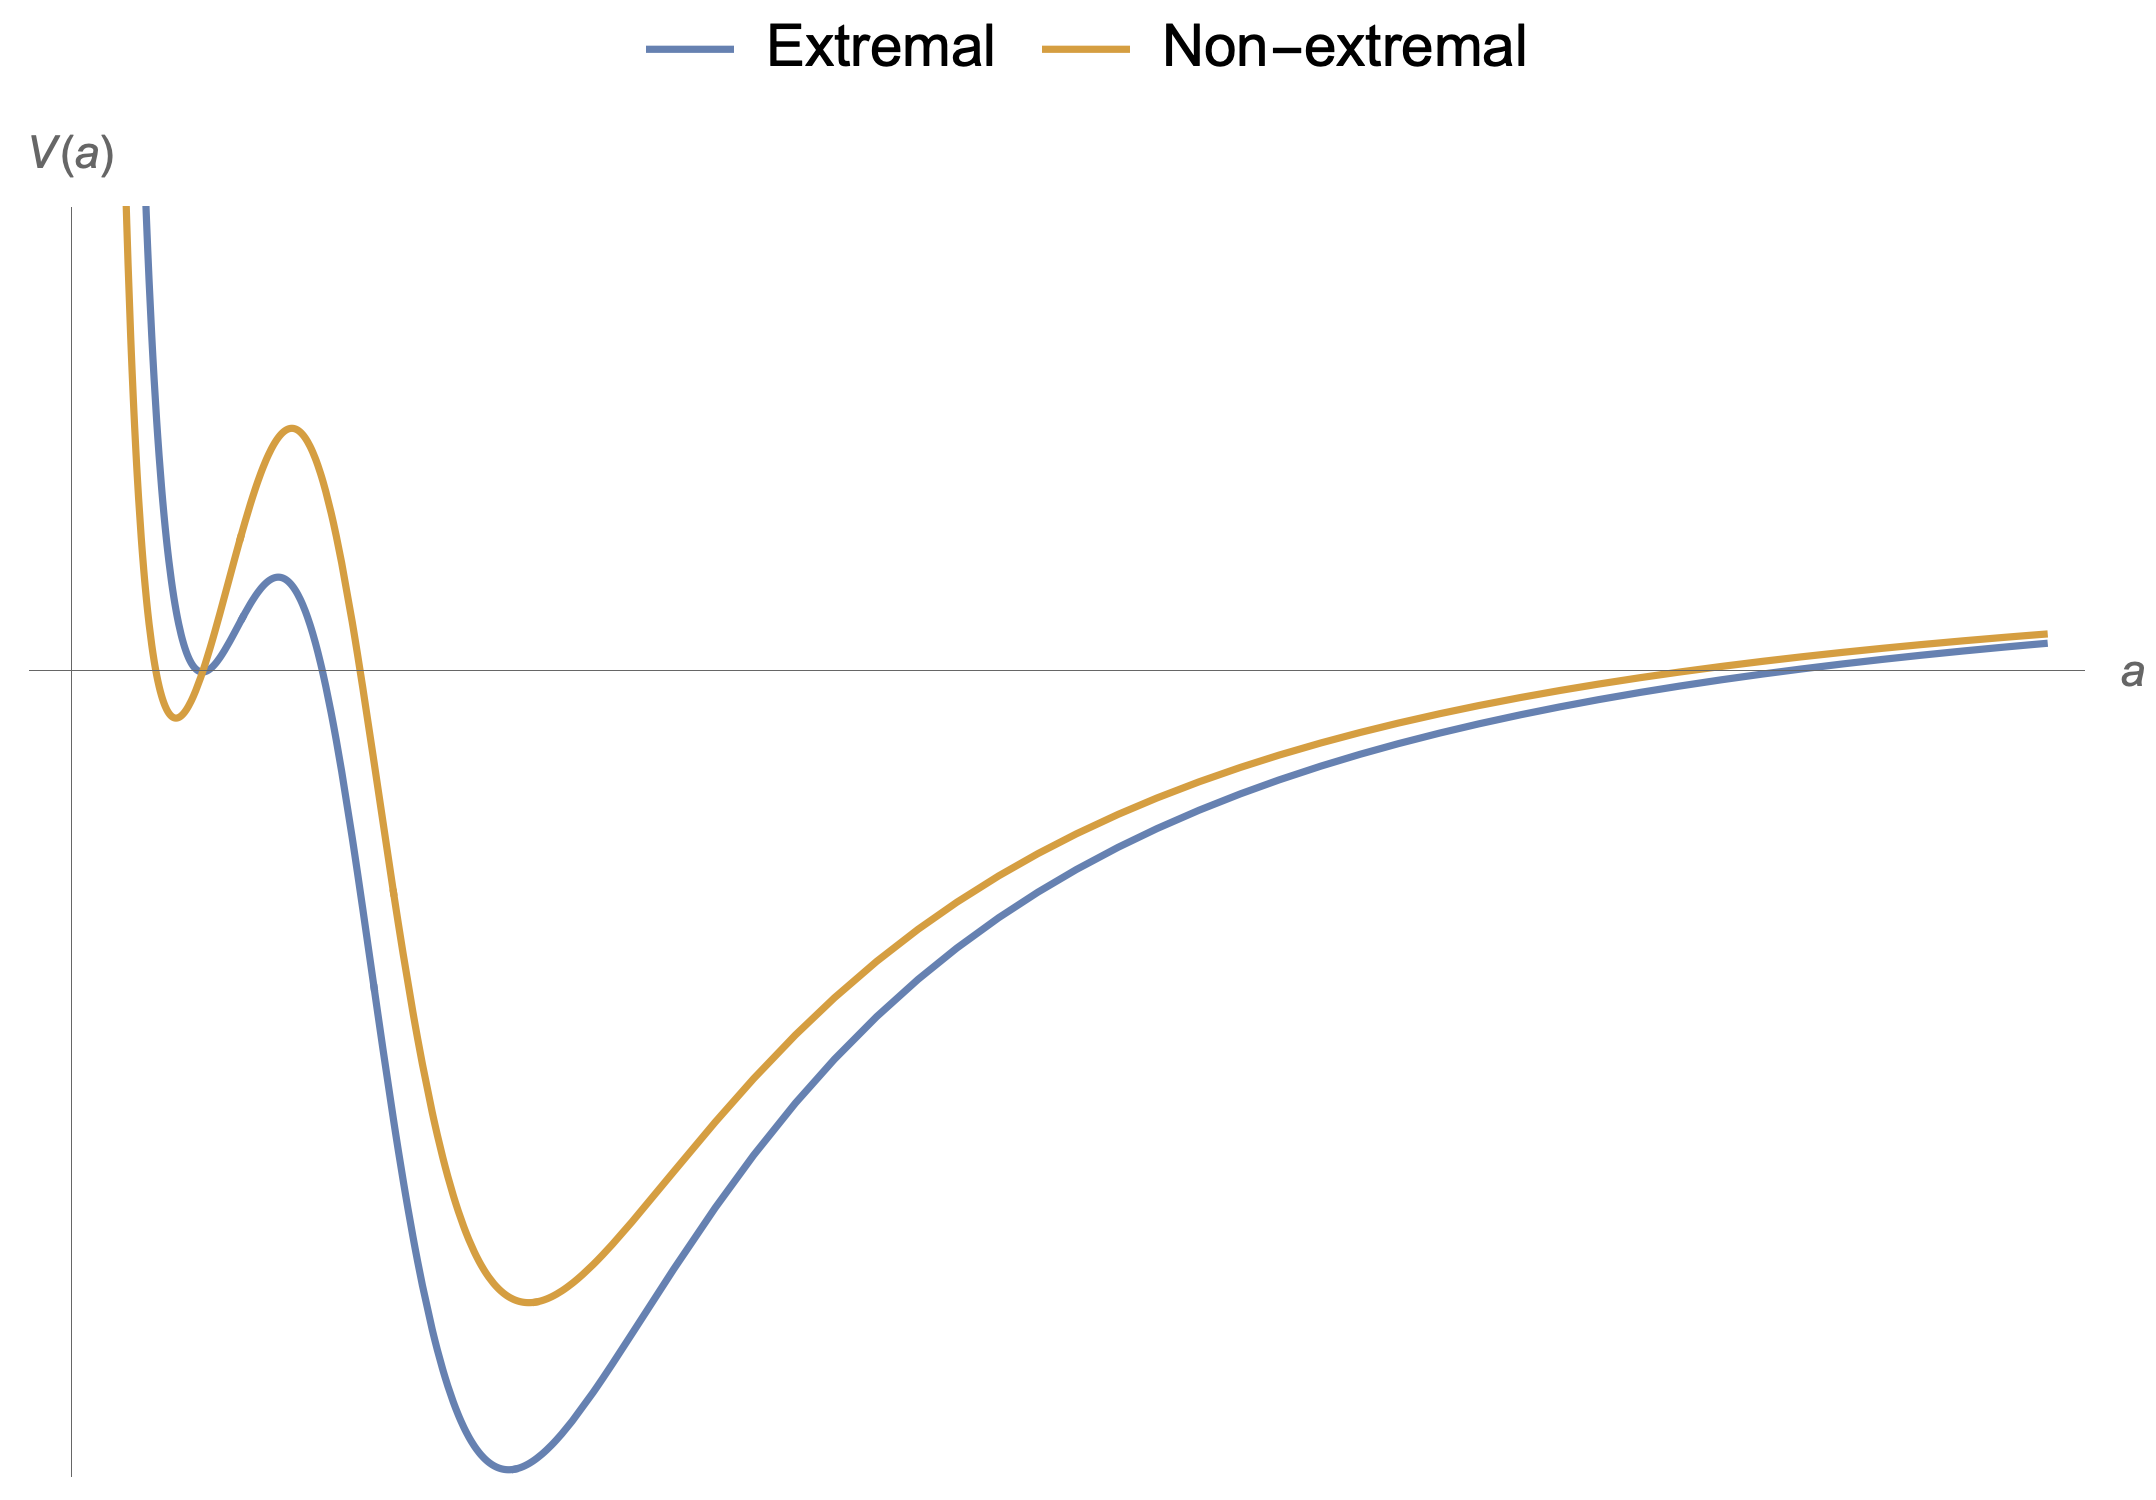
\includegraphics[width=12cm]{Figures/db_pot.png}
    \caption{The potential controlling the dynamics of the embedded four dimensional universe.}
    \label{fig: full_potential}
\end{figure}
\textcolor{red}{TRANSFORM TO SVG !!}\\
There are three (four) special points to consider in figure (\ref{fig: full_potential}):
\begin{itemize}
    \item Both horizons $\{a_{h}, a_{H}\}$ (first two roots in the non-extremal case): They respectively correspond to the inner and outer horizons of the Reisser-Nordström black hole. In the extremal case, both horizons coincide, which corresponds to the first root of the blue plot. 
    \item The nucleation point $\{a_{\text{nuc}}\}$ ($2^{\text{nd}}$ or $3^{\text{rd}}$ roots, respectively): This is the value of $a$ at which the $D_{3}$ brane (i.e. the four-dimensional universe) will nucleate. The region between $a_{H}$ and $a_{\text{nuc}}$ is the classical forbidden region that the brane will have to tunnel through. More to be discussed in section (\ref{sec: quantum_bubbles}).
    \item The maximal size $\{a_{b}\}$ of the collapsing universe:  This is given by the last root of the potential $V(a)$. At this point, the size of the bubble is maximal, and the four dimensional universe, without positive dark energy density, but equipped with positive curvature, will reach its maximum size and start contracting, in the form of a bouncing cosmology.
\end{itemize}
But, What different features are controlled by which parameters? By construction, the potential (\ref{eq: potential_extremal_subs}) goes to 1 when the scale factor $a\rightarrow \infty$. The AdS scale $k^{-1}$ is in charge of controlling the overall value of the potential (i.e. basically scaling the $y$-axis). The angular momentum of the brane $J_{C}$ will regulate the barrier of the potential.

The potential described in Eq. (\ref{eq: potential_extremal_subs}) lacks a sustained cosmological constant and experiences only a fraction of an e-folding just after creation. The expansion rate vanishes at nucleation, the universe then accelerates for a short time after which it enters a decelerated phase. Since the curvature is positive, and there is no asymptotic cosmological constant, the universe will eventually stop expanding and start to contract, entering an oscillating phase with repeated bounces. 

Of course, this is not the desired fate for the dark bubble model in its stringy embedding. It is our aim to find a low-dimensional model capable of describing dark energy derived from string theory. Does previous computations indicate that the dark bubble model embedding should be ruled out? Absolutely not. All stringy computation so far have been performed assuming the brane to be BPS, although the ten-dimensional ambient space hosting it has broken supersymmetry. This will be taken into account in the incoming sections.


\subsection{Higher curvature corrections to the rescue}
Point to the fact that previous EOM has no CC. Discuss about how to obtain it and elaborate on all pieces in the game. End with the famous $1/N$ corrections that transform in CC. (First part of 5th paper)
\subsection{Energy scales from Dark Bubble embedding: A new hope}\label{subsec: energy_scale}
Compare to observed CC and obtain $N$ to fix all scales. Discuss and defend the size of extra dimensions and the stringy scales.